%-------------------------------------------------------------------------------
\documentclass[twocolumn]{article}

%-------------------------------------------------------------------------------
% Packages
\usepackage[portuguese]{babel}
\usepackage{environ}
\usepackage[margin=2cm]{geometry}
\usepackage{graphicx}
\usepackage{hyperref}
\usepackage{minted}
\usepackage{xcolor}

%-------------------------------------------------------------------------------
% User-commands
\newcommand{\todo}[1]{{\color{red}{#1}}}

\NewEnviron{superframe}{%
    \begin{center}
        \fbox{\setlength{\fboxsep}{1em}\fbox{\parbox{5.5in}{%
            \BODY{}
        }}}
    \end{center}
}

\newmintedfile[textfile]{text}{autogobble, breaklines}

%-------------------------------------------------------------------------------
% Project configs
\title{Relatório de I.A.: Sistemas Fuzzy (Trabalho 4)}
\author{Cauê Baasch de Souza \\
        João Paulo Taylor Ienczak Zanette}
\date{\today}

%-------------------------------------------------------------------------------
\begin{document}
    \maketitle{}

    \section{O ``Fuzzy Truck''}

    No problema ``Fuzzy Truck'', é necessário definir parâmetros, saídas e
    regras de um sistema Fuzzy para fazer um caminhão, andando de ré,
    estacionar em uma doca considerando um espaço 2D sem obstáculos. Como
    restrições do problema, o caminhão possui velocidade constante (com exceção
    de que ele para quando está suficientemente próximo do espaço que delimita
    a vaga) e suas únicas ações possíveis são: girar o volante para a esquerda
    (indicado pelo valor -1), manter a direção atual do caminhão (valor 0) e
    girar o volante para a direita (valor 1).

    O espaço por onde o caminhão anda é delimitado pelas coordenadas X e Y
    variando de 0 a 1 com um pequeno limiar extra (com exceção de valores de $Y
    > 1$). Ao se passar dessa delimitação, a simulação é encerrada e uma
    pontuação é dada considerando o número de passos dados, o ângulo final do
    caminhão e a distância até a doca, que está centralizada no ponto $(0.5,
    1)$.

    \section{Resolvendo o problema do ``Fuzzy Truck''}

    \subsection{Entradas utilizadas e Conjuntos Fuzzy}

    Foram utilizadas três entradas simples: as coordenadas $X$ e $Y$ e o ângulo
    do caminhão (em graus). Os conjuntos fuzzy (visualizáveis na
    Figura~\ref{fuzzy-sets}) foram definidos pensando em:

    \begin{figure}[ht]
        \centering{}
        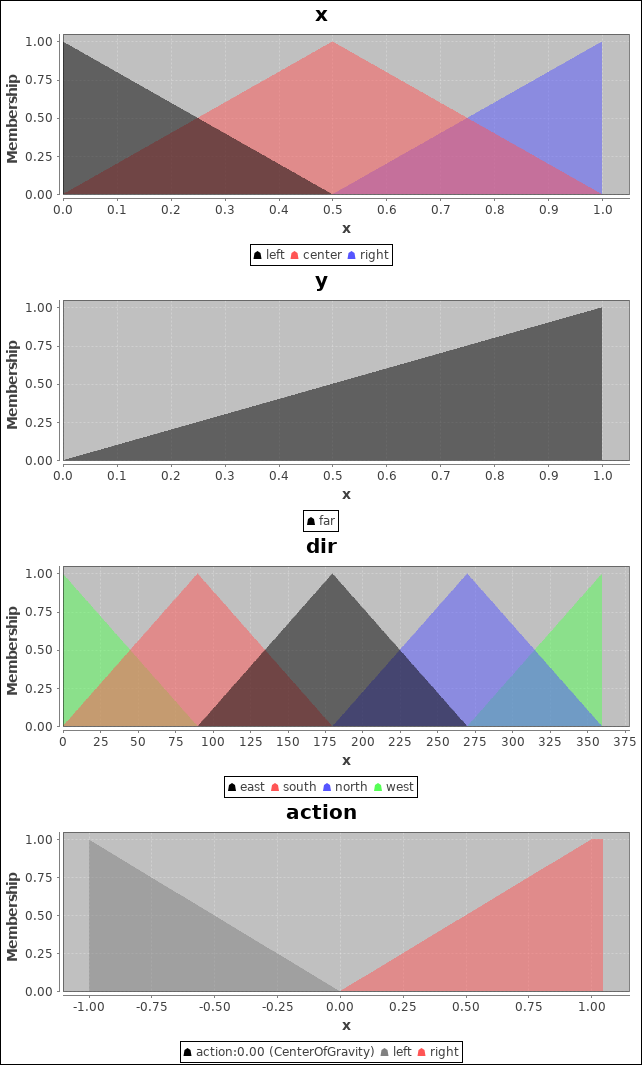
\includegraphics[keepaspectratio,width=.5\textwidth]{img/truck-fuzzifiers}
        \caption{%
            Conjuntos Fuzzy para variáveis de entrada e saída do ``Fuzzy
            Truck''.\label{fuzzy-sets}
        }
    \end{figure}

    \begin{itemize}
        \item O quão longe o caminhão está horizontalmente, separando em:
            ``muito para a esquerda'', ``muito para a direita'' e
            ``centralizado'';
        \item O quão longe o caminhão está verticalmente, separando em: ``muito
            longe'' e ``próximo'';
        \item A direção do caminhão, separada em: norte, sul, leste e oeste.
    \end{itemize}

    \subsection{Regras utilizadas e Defuzzificação}

    Por simplicidade, as regras definidas foram:

    \begin{itemize}
        \item Muito para a esquerda $\land$ Norte $\rightarrow$ Virar para a
            direita
        \item Muito para a esquerda $\land$ Muito longe $\land$ Leste
            $\rightarrow$ virar para a direita
        \item Muito para a esquerda $\land$ Muito longe $\land$ Sul
            $\rightarrow$ virar para a esquerda
        \item Centralizado $\land$ Oeste $\rightarrow$ Virar para a esquerda
        \item Centralizado $\land$ Norte $\rightarrow$ Virar para a esquerda
        \item Centralizado $\land$ Leste $\rightarrow$ Virar para a direita
        \item Muito para a direita $\land$ Norte $\rightarrow$ Virar para a
            esquerda
        \item Muito para a direita $\land$ Muito longe $\land$ Oeste
            $\rightarrow$ virar para a esquerda
        \item Muito para a direita $\land$ Muito longe $\land$ Sul
            $\rightarrow$ virar para a direita
    \end{itemize}

    A ação é defuzzificada dos conjuntos ``virar para a direita'' ou ``virar
    para a esquerda'' para um valor no intervalo $[-1, 1]$. Um conjunto para a
    ação de ``não virar'' foi experimentado, mas ele se mostrou desnecessário e
    ineficiente, porque uma decisão que deveria ter um alto grau de pertinência
    para ``não virar'' já terá, de acordo com as regras, um baixo grau de
    pertencimento aos conjuntos respectivos às outras ações. Consequentemente,
    tal decisão já terá um valor próximo do zero esperado.

    \section{Conclusões e considerações}

    Devido à vontade de aventura, os alunos decidiram utilizar o gerador de
    código C++ a partir de FCL (linguagem de descrição de sistemas Fuzzy) pelo
    jFuzzyLogic (biblioteca e programa para funcionalidades relacionadas a
    lógica Fuzzy, incluindo geração de gráficos). Um pouco fora do esperado,
    foram feitos alguns passos extras como: melhoria do código gerado,
    separação das declarações em header, e implementação simples de uma API
    Socket em C++. Porém, tendo esses passos prontos, os ajustes e criação das
    regras e parâmetros do sistema para o FuzzyTruck foram mais triviais. Como
    FCL obriga a enumeração de regras, para melhorar a produtividade criou-se
    um pequeno script em Python que gerava o arquivo FCL a partir de regras
    definidas em uma lista de \texttt{Rule}s (uma tupla com os valores
    esperados e o valor de saída para a regra).

    Da parte da definição das regras, diferentes abordagens foram tomadas
    tentando ser o mais restritivo possível: utilização de pontos colaterais
    (totalizando 8 direções) e definindo regras para cada caso (muito longe, no
    centro ou perto em Y, combinando com se está à esquerda, centro ou direita
    em X, combinando com cada uma das direções possíveis). Para cada mudança
    nas regras, o caminhão se comportava com desempenho muito bom (às vezes
    melhor do que a versão final deste trabalho) para um mesmo conjunto de
    valores de entrada, porém em outro o desempenho era péssimo. Depois de
    vários testes e regras específicas criadas, decidiu-se remodelar as
    entradas bem como seus conjuntos fuzzy e então redefinir regras simples e
    diretas. Com essa última mudança, os resultados se tornaram muito mais
    plausíveis para uma boa parte dos casos não extremos (como iniciar-se muito
    próximo da doca em Y, porém muito longe em X). Tentativas de adicionar
    novas regras voltaram ao mesmo comportamento de antes: melhoravam um pouco
    em alguns pontos, pioravam muito mais em outros.

    Sendo assim, é possível (e mais aconselhável) confiar no sistema Fuzzy para
    escolher as ações em resultados intermediários, se preocupando apenas com
    pontos estratégicos dos conjuntos Fuzzy em vez de deixá-los densos e
    extremamente detalhistas.

    \bibliographystyle{unsrt}
    \bibliography{refs}
    \nocite{*}
\end{document}
